\documentclass[physics_notes.tex]{subfiles}
\begin{document}
\section{Aula 10 - 24/04/2023}
\subsection{O que esperar?}
\begin{itemize}
	\item Continuação de Dinâmica;
	\item Tipos de forças.
\end{itemize}
\subsection{Motivação}
Neste resumo, discutiremos diferentes tipos de forças em física, suas fórmulas e algumas propriedades. Elas serão abordadas ao longo
das próximas aulas, não apenas nesta primeira. \textbf{Nota ao Leitor: as fórmulas aqui apresentadas são apenas
	para o módulo das forças, mas esta palavra foi omitida para não ficar muito repetitivo. As forças são estudadas vetorialmente,
	não esqueça-se disto.}

A força gravitacional é a atração entre dois objetos devido à sua massa. A fórmula da força gravitacional é:

\begin{equation}
	F_g = G \frac{m_1 m_2}{r^2}
\end{equation}

onde $F_g$ é a força gravitacional, $G$ é a constante gravitacional, $m_1$ e $m_2$ são as massas dos dois objetos e $r$ é a distância entre seus centros de massa.
\begin{center}
	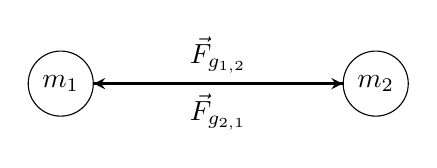
\begin{tikzpicture}
		\node[draw, circle] (m1) at (0,0) {$m_1$};
		\node[draw, circle] (m2) at (4,0) {$m_2$};
		\draw[->, >=stealth, thick] (m1) -- node[above] {$\vec{F}_{g_{1,2}}$} (m2);
		\draw[->, >=stealth, thick] (m2) -- node[below] {$\vec{F}_{g_{2,1}}$} (m1);
	\end{tikzpicture}
\end{center}

A força normal é a força que um objeto exerce perpendicularmente à sua superfície de contato com outro objeto. Esta força é responsável por impedir que os objetos atravessem uns aos outros. A força normal tem módulo igual à componente do peso do objeto perpendicular à superfície.

\begin{center}
	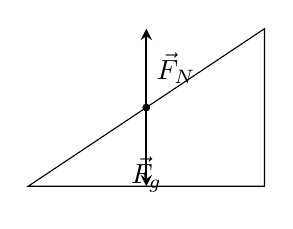
\begin{tikzpicture}
		\draw (0,0) -- (3,0) -- (3,2) -- cycle;
		\draw[->, >=stealth, thick] (1.5, 1) -- node[right] {$\vec{F}_N$} (1.5, 2);
		\draw[->, >=stealth, thick] (1.5, 1) -- node[below] {$\vec{F}_g$} (1.5, 0);
		\node at (1.5, 1) [circle, fill, inner sep=1pt] {};
	\end{tikzpicture}
\end{center}

A força de atrito é a força que age oposta ao movimento relativo entre duas superfícies em contato. Existem dois tipos de força de atrito: estático e cinético.
A força de atrito estático age entre duas superfícies em repouso relativo e é responsável por impedir que objetos comecem a se mover. A força de atrito estático pode variar de zero até o valor máximo dado por:

\begin{equation}
	F_{s_{max}} = \mu_s F_N
\end{equation}

onde $F_{s_{max}}$ é a força de atrito estático máxima, $\mu_s$ é o coeficiente de atrito estático e $F_N$ é a força normal.
A força de atrito cinético age entre duas superfícies em movimento relativo e é responsável por reduzir a velocidade dos objetos. A força de atrito cinético é dada por:

\begin{equation}
	F_k = \mu_k F_N
\end{equation}

onde $F_k$ é a força de atrito cinético, $\mu_k$ é o coeficiente de atrito cinético e $F_N$ é a força normal.
\begin{center}
	\begin{tikzpicture}
		\draw (0,0) -- (4,0);
		\node[draw, rectangle] (box) at (2,0.5) {Caixa};
		\draw[->, >=stealth, thick] (box.north) -- ++(0,1.5) node[above] {$\vec{F}_N$};
		\draw[->, >=stealth, thick] (box.south) -- ++(0,-1.5) node[below] {$\vec{F}g$};
		\draw[->, >=stealth, thick] (box.west) -- ++(-1.5,0) node[left] {$\vec{F}{k}$};
	\end{tikzpicture}
\end{center}

Estas duas últimas forças, ou seja, forças normal e atrito, encaixam-se na classe de forças de contato.

A força tensional é a força que atua ao longo de um cabo, corda ou fio quando esticado por forças opostas aplicadas em suas extremidades. A força tensional é transmitida ao longo do comprimento do cabo, corda ou fio.
\begin{center}
	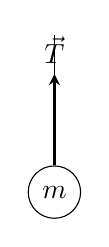
\begin{tikzpicture}
		\node[draw, circle] (mass) at (0,-1) {$m$};
		\draw[->, >=stealth, thick] (mass) -- ++(0,1.5) node[above] {$\vec{T}$};
		\draw (0,0) -- (0,1);
	\end{tikzpicture}
\end{center}

A força elástica é a força de restituição que atua quando um objeto é deformado, como uma mola esticada ou comprimida. A força elástica segue a Lei de Hooke:

\begin{equation}
	F_e = -k \Delta x
\end{equation}

onde $F_e$ é a força elástica, $k$ é a constante elástica e $\Delta x$ é o deslocamento da posição de equilíbrio da mola.
\begin{center}
	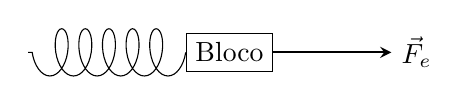
\begin{tikzpicture}
		\node[draw, rectangle] (block) at (0,0) {Bloco};
		\draw[->, >=stealth, thick] (block.east) -- ++(1.5,0) node[right] {$\vec{F}_e$};
		\draw[decoration={coil, segment length=3mm, aspect=0.5, amplitude=3mm}, decorate] (block.west) -- ++(-2,0);
	\end{tikzpicture}
\end{center}

A força de arrasto é a força de resistência que um objeto experimenta ao se mover através de um fluido (líquido ou gás). A força de arrasto é proporcional ao quadrado da velocidade do objeto em relação ao fluido e é dada por:

\begin{equation}
	F_D = \frac{1}{2} \rho v^2 C_D A
\end{equation}

onde $F_D$ é a força de arrasto, $\rho$ é a densidade do fluido, $v$ é a velocidade do objeto, $C_D$ é o coeficiente de arrasto e $A$ é a área da seção transversal do objeto.

\begin{center}
	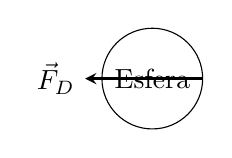
\begin{tikzpicture}
		\node[draw, circle] (sphere) at (0,0) {Esfera};
		\draw[->, >=stealth, thick] (sphere.east) -- ++(-1.5,0) node[left] {$\vec{F}_D$};
	\end{tikzpicture}
\end{center}

\subsection{Tipos de Força}
\subsubsection{As Quatro Forças Fundamentais de Forma Breve}
O primeiro tipo de força que veremos é a Interação gravitacional. Ela ocorre na forma da interação de corpos massivos,
sendo representada pela força peso. Além disso, ela é uma força atrativa e de longo alcance. Em particular, o módulo da
força gravitacoinal é
$$
	|\vec{F}_{21}| = |\vec{F}_{12}| = \frac{Gm_{1}m_{2}}{r^{2}}.
$$
Aqui, G é a constante de gravitacional, cujo valor é $G=6.67 \cdot 10^{-11}Nkg^{-2}m^{2}.$

A segunda forma de interação é a eletromagnética, estando presente no contexto de partículas carregadas. Ela será
atrativa dado que as duas cargas $q_{1}, q_{2}$ possuam sinais opostos ($q_{1}\cdot q_{2}<0$) e repulsivas caso possuam sinais
iguais ($q_{1}\cdot q_{2}>0$). Seu módulo é dado por
$$
	|\vec{F}_{12}|=|\vec{F}_{21}|=k\frac{q_{1}q_{2}}{r^{2}}.
$$

Outra força que existe é a interação forte, que age em curto alcance, aproximadamente do tamanho do núcleo atômico.
Ela é responsável por manter os prótons e neutron no núcleo.

A última força fundamental é a interação fraca, sendo uma que ocorre em curtíssimo alcance e presente em alguns
decaimento radioativos.

Em dinâmica, estudaremos principalmente interações gravitacionais na forma da Força Peso e interações eletromagnéticas,
que se manifrestarão nas formas da força normal, força de tração, força de atrito, entre outras.

\subsubsection{Força Peso}
A força peso é descrita como a atração de um corpo por um objeto celeste quando o corpo está em sua superfície.
Como vimos previamente, ela é dada, na Terra, por
$$
	F_{g} = \frac{GMm}{R_{T}^{2}} = mg.
$$
Isso ajuda-nos a descobrir, em particular, como obter o valor da aceleração na superfície. Considerando a massa
de humanos como desprezível em comparação à da Terra, obtemos
$$
	g = \frac{GM_{T}}{R_{T}^{2}}\approx 9.81m/s^{2}.
$$
A força peso que iremos considerar é definida como $\vec{P} = m \vec{g}$. Consideremos um exemplo.

\begin{example}
	Considere uma pessoa pulando. A Terra exerce uma força atrativa nela de volta para a superfície, a força Peso, tal que
	a força resultante nela é dada por
	$$
		\vec{F}_r = \vec{P} = m \vec{g} - m \vec{a}.
	$$
	Caso a pessoa esteja na superfície, ela estará em equilíbrio, ou seja, $\vec{F}_{r} = 0.$ Com isso, segue que
	$$
		\vec{F}_{r} = \vec{P} + \vec{N} = 0.
	$$
	Essa força oposta à Peso, que denotamos por N, será estudada a seguir.
\end{example}

\subsubsection{Força Normal}
A força normal é a resultante do contato dos corpos, com direção perpendicular às superfícies de contato. Ela não
possui uma fórmula exata, pois é uma interação muito complexa relacionada a moléculas e forças eletromagnéticas.
\begin{example}
	Considere uma escada encostada a uma parede. Então, haverá uma força normal conseguinte do contato entre a escada
	e a parede perpendicular à parede.
	\begin{center}
		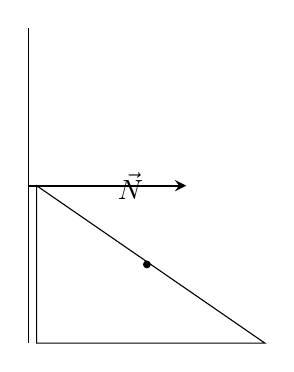
\begin{tikzpicture}
			\draw (0,0) -- (0,4);
			\draw[->, >=stealth, thick](0, 2)-- node[right] {$\vec{N}$} (2, 2);
			\draw (3,0) -- (0.1,0) -- (0.1,2) -- cycle;
			\node at (1.5, 1) [circle, fill, inner sep=1pt] {};
		\end{tikzpicture}
	\end{center}
\end{example}
\begin{example}
	Considere um bloco no elevador. Qual é a força normal? Na situação (a), considere-o [o elevador] parado. Na
	situação (b), ele possui velocidade constante. No caso (c), o elevador está acelerando para cima. Finalmente,
	no item (d), o elevador acelera para baixo.

	Estando ele parado, a aceleração e a velocidade são nulos. Com isso, sabe-se o valor da resultante:
	$$
		\vec{F}_{r} = m \vec{a} = \vec{0}.
	$$
	Observando a esquemática do problema, nota-se que nada ocorre no eixo x, além de que $\vec{a}_{x} = F_{r}^{x} = 0.$
	No entanto, com relação ao eixo y, observamos que, apesar de $\vec{a}_{y} = F_{r}^{y} = 0,$ existem forças atuando
	sobre o bloco. Assim,
	$$
		0 = F_{r}^{y} = -P + N = -mg + N = 0 \Rightarrow N = mg = P.
	$$

	Quanto à situação (b), note que, novamente, a força resultante será 0, pois a velocidade é constante.
	analisando as forças em y, assim, obtemos o mesmo resultado que no item (a):
	$$
		0 = F_{r}^{y} = -P + N \Rightarrow N = P = mg.
	$$

	No item (c), como o elevador está acelerado, existe uma aceleração para o bloquinho, tal que
	$$
		\vec{F}_{r} = m \cdot \vec{a} \neq 0.
	$$
	No eixo y, as duas forças continuam as mesmas, ou seja,
	$$
		F_{r}^{y} = -P + N = m \cdot a\neq 0.
	$$
	Assim, a força normal será dada por
	$$
		N = m(a + g).
	$$

	Por fim, no caso (d), novamente, há uma aceleração, então a resultante é não-nula. No entanto, como a aceleração é para baixo,
	$$
		\vec{F}_{r} = m \cdot \vec{(-a)}\neq 0.
	$$
	Com isso,
	$$
		F_{r}^{y} = -P + N = m \cdot \vec{(-a)} \Rightarrow N = m(g - a).
	$$
\end{example}
\begin{example}
	Considere o um plano inclinado e um bloco deslizando nele. Qual é a aceleração $\vec{a}?$
	\begin{center}
		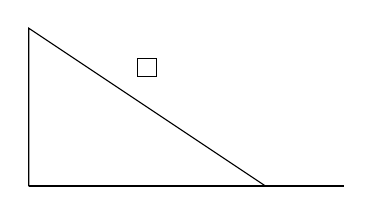
\begin{tikzpicture}
			\draw (0,2) -- (3,0) -- (0,0) -- cycle;
			\node[rectangle, draw] at (1.5,1.5){};
			\draw[thick] (0, 0) -- (4, 0);
		\end{tikzpicture}
	\end{center}
	Temos $\vec{N} = |\vec{N}|\hat{j}, |\vec{P}|=mg.$ Lembre-se que
	$$
		\left\{\begin{array}{ll}
			P_{x}' = |\vec{P}|\sin{\theta} \\
			P_{y}' = |\vec{P}|\cos{\theta}
		\end{array}\right.
	$$
	Com isso, as componentes de força são
	\begin{align*}
		 & x') \Rightarrow F_{r}^{x'} = P_{x'} = |\vec{P}|\sin{\theta} = ma_{x'}      \\
		 & y') \Rightarrow F_{r}^{y'} = -P_{y'} + N = -|\vec{P}|\cos{\theta} + N = 0.
	\end{align*}
	Desta última equação, tiramos que a força normal é $N = |\vec{P}|\cos{\theta} = mg\cos{\theta}.$ Além disso,
	da primeira equação, temos
	$$
		a_{x}' = \frac{mg\sin{\theta}}{m} = g\sin{\theta}.
	$$
	Portanto, $\vec{a} = a_{x'}\hat{i} = g\sin{\theta}\hat{i}.$
\end{example}
\begin{example}
	Exemplo 4.7 do Tipler: Temos $v_{y}\leq 2.5m/s$ e uma altura de 1m. Pergunta-se: Qual é o maior ângulo possível?

	Após deslocar-se em $\Delta x$, o pacote tem $v_{x'}$ dado por
	$$
		v_{x'}^{2} = v_{0_{x'}}^{2} + 2 a_{x'}\Delta x' = 2a_{x'}\Delta x' \Rightarrow v_{x'}^{2} = \frac{2g\sin{\theta}h}{\sin{\theta}} = 2gh.
	$$
	Logo, $v_{x'} = \sqrt[]{2gh}$. Assim,
	$$
		\left\{\begin{array}{ll}
			v_{x} = v_{x}'\cos{\theta} \\
			v_{y} = v_{x'}\sin{\theta}\leq 2.50m/s.
		\end{array}\right.
	$$
	Disso segue que
	$$
		\sqrt[]{2gh}\sin{\theta}\leq 2.5m/s \Rightarrow \sqrt[]{2gh}\sin{\theta_{max}} = 2.5m/s
	$$
	Portanto, $\theta_{max} = 34.4^{\circ}.$
\end{example}
\end{document}
